%\documentclass[document.tex]{subfiles}
%\begin{document}

%%{\section{The Purpose of the Project}\label{sec:Purpose}}
\subsection{Purpose of the project}
\edcomm{YS}{Added the ``AMMBR section'' based on comments from Dr. Kahl. He has verified the section, I'll follow up with a proof read and other section of this document}

Ampersand follows a \emph{rule based} design principle. Rules are integral to an organization
and these are based on some principles and guidelines set by the organization.
Ampersand uses an ECA ( Event - Condition - Action \edcomm{WK}{IMO,
  either ``Event-Condition-Action'' or ``Event --- Condition --- Action''}) approach to make sure all rules are satisfied. An ideal information infrastructure supports employees and other stakeholders to maintain the rules of the business. To maintain a rule means to prevent or correct all violations that might occur due to any external or internal factor.
 
 A large portion of the Ampersand system is already in place; the primary focus of this project was to
augment Ampersand with increased capabilities for automation. The module ``Automatically Fix Violations'' in Figure ~\ref{fig:EFAproject} represents the EFA project and where it fits in the current version of Ampersand.
\edcomm{JG}{Could you mention what "this problem" is? When you read it, 'this' 
seems to refer back to something specific and I'm not sure what, it seems 
confusing } \edcomm{YS} {Addressed}
Ampersand relies on the AMMBR \citep{Ampersand} algorithm to help fix these data violations.
The role 
of the AMMBR method in Ampersand \edinsert{WK}{is to} automatically generate correction methods that 
help maintain these business rules. In AMMBR, human involvement is only limited 
to representing rules (in the ADL files).
\edchange{WK}{%
While the Ampersand software still 
remains in development phase, there is no way of checking the correctness of 
the AMMBR method at a low level.
}{%
Before our current project was started, there was no way of actually
applying the AMMBR-generated ECA rules to rule-violating database states.
There was therefore also no means to test whether AMMBR is producing
appropriate ECA rules.
}%edchange
\edchange{WK}{%
Previously, the Exec Engine was used to 
maintain these business rules, that required direct injection of SQL 
hand-written as PHP strings. 
}{%
The current state of Ampersand uses, as a work-around, the so-called
``Exec engine'', which makes maintenance of business rules possible
via direct injection of SQL hand-written as PHP strings.
}%edchange

The EFA project, an extension to the Ampersand system, allows us to evaluate 
the correctness of the Action \edcomm{WK}{``the Action'' sounds
  somewhat strange to me} according to the ECA rules.
This will 
allow us to automatically rehabilitate \edcomm{WK}{???} existing system data while 
maintaining the information system according to user specifications. 
Furthermore, EFA permits us to automate the restoration of system invariants, 
and create a program which helps Ampersand to make the most efficient choice 
regarding how to proceed on a case-by-case basis. \edcomm{WK}{Has this
  previous sentence survived from an earlier document? I guess it does
  not really apply to your final state?}
The ECA rules, which act as an 
input to the EFA project, are translated into human-readable SQL.
This can later be viewed in the command line \edcomm{WK}{This probably
  does not belong here, but in some ``user guide'' section.}
using the ``\verb|--print-eca-info|'' flag,
which is written out in one of the artifacts.
The generated SQL queries not only 
allow  the correctness of AMMBR to be checked, but also help in the 
identification of patterns and unreachable states. Therefore, EFA will be an 
essential tool for testing the AMMBR algorithm.


\begin{figure}[!htb]
\begin{center}
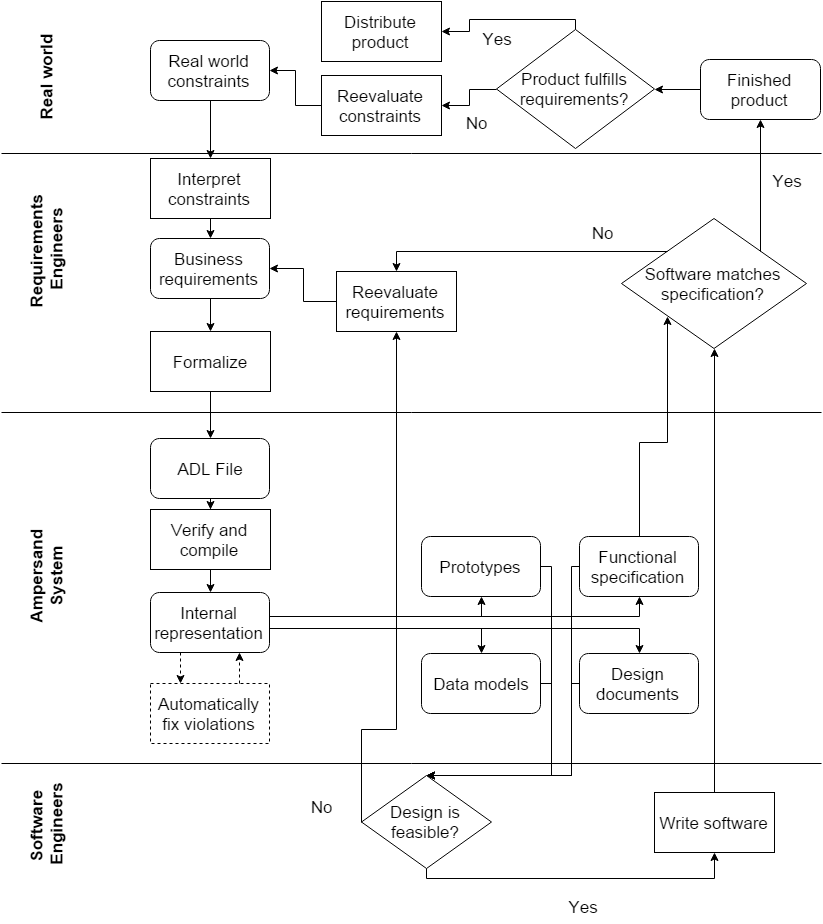
\includegraphics[width=\textwidth]{../figures/business_process}
\caption{Business process diagram representing EFA project represented as a dashed box}~\label{fig:EFAproject}
\end{center}
\end{figure}

 \subsection{The Stakeholders and the intended audience}\label{sec:Stakeholders}
The stake holders of Ampersand are:

\begin{itemize}
	\item \textbf{Ampersand Designers}: Responsible for maintaining and developing Ampersand.
	\item \textbf{The Customer}: The end users of Ampersand
          \edcomm{WK}{that is, requirements engineers using Ampersand
            to generate prototypes, as opposed to the end-users of
            Ampersand-generated prototypes} will benefit from the EFA
          project.
          This will decrease the amount of time 
Ampersand users spend manually inserting PHP code to restore system invariants. 
\end{itemize}

This document is designed to help introduce \eddelete{WK}{new} Ampersand users to EFA 
(ECA rules for Ampersand). It provides a basic structure that allows 
individuals to quickly access the information they seek. 
